%% ============================================================
%%  docs/octree_pt.tex
%%  Tradução PT-PT: Octrees SDF Adaptativas para CSG de
%%  Terreno em Tempo Real e Geração de Malhas Surface Nets
%% ============================================================
\documentclass[10pt,a4paper]{article}

\usepackage[T1]{fontenc}
\usepackage[utf8]{inputenc}
\usepackage{lmodern}
\usepackage{microtype}
\usepackage{geometry}
\geometry{left=2.5cm, right=2.5cm, top=2.8cm, bottom=2.8cm}

\usepackage{amsmath,amssymb,amsthm}
\DeclareMathOperator*{\argmin}{arg\,min}
\usepackage{xcolor}
\usepackage{graphicx}
\usepackage{booktabs}
\usepackage{hyperref}
\usepackage{cleveref}
\usepackage{float}
\usepackage{caption}
\usepackage{subcaption}
\usepackage{enumitem}
\usepackage{multicol}

%% ---- TikZ ---------------------------------------------------
\usepackage{tikz}
\usetikzlibrary{
  arrows.meta, positioning, shapes.geometric, fit, calc,
  decorations.pathreplacing, backgrounds, patterns
}
\usepackage{pgfplots}
\pgfplotsset{compat=1.18}

%% ---- Algorithms --------------------------------------------
\usepackage{algorithm}
\usepackage{algpseudocode}

%% ---- Listings ----------------------------------------------
\usepackage{listings}
\lstdefinestyle{cpp}{
  language=C++,
  basicstyle=\ttfamily\small,
  keywordstyle=\color{blue!70!black}\bfseries,
  commentstyle=\color{gray!60},
  stringstyle=\color{orange!80!black},
  numberstyle=\tiny\color{gray},
  numbers=left,
  numbersep=6pt,
  breaklines=true,
  tabsize=2,
  showstringspaces=false,
  frame=single,
  rulecolor=\color{gray!30},
  backgroundcolor=\color{gray!4},
  captionpos=b
}
\lstset{style=cpp}

%% ---- Theorem environments ----------------------------------
\newtheorem{definition}{Definição}
\newtheorem{remark}{Observação}

%% ---- TikZ helpers ------------------------------------------
% Ajuda para projeção oblíqua: (x,y,z) -> 2D com z para dentro da página
% proj_x = x + 0.40*z,  proj_y = y + 0.30*z
\newcommand{\prjnode}[4]{% \prjnode{nome}{x}{y}{z}
  \pgfmathsetmacro{\px}{#2 + 0.40*(#4)}
  \pgfmathsetmacro{\py}{#3 + 0.30*(#4)}
  \coordinate (#1) at (\px, \py);
}

%% ============================================================
\title{%
  \textbf{Octrees SDF Adaptativas para CSG de Terreno em Tempo Real e Geração de Malhas Surface Nets}\\[4pt]
  {\large Estrutura, Operações e Extração de Triângulos}
}
\author{Relatório Técnico do Motor Vulkan}
\date{2026}

\begin{document}
\maketitle

\begin{abstract}
Descrevemos o desenho e a implementação de uma octree adaptativa que
serve como a principal estrutura de dados espaciais para geometria
sólida construtiva (CSG) em tempo real em terreno definido por funções
de distância sinalizada (SDF). A octree guarda amostras SDF nos cantos
de cada nó, permitindo classificação eficiente de regiões (\emph{Vazio},
\emph{Sólido}, \emph{Superfície}), CSG dinâmico através de um percurso
recursivo chamado \emph{shape}, e simplificação com base no nível de
detalhe (LOD). A extração da malha usa um algoritmo chamado
\emph{surface nets}: para cada aresta alinhada aos eixos que atravessa
a superfície zero da SDF, um polígono duplo é montado a partir das
quatro células que partilham essa aresta. Uma regra de propriedade
impede a emissão duplicada entre limites de células, e a orientação
dos vértices é determinada apenas pelo sinal da SDF nos extremos da
aresta. A malha resultante é enviada diretamente para um renderizador
Vulkan que usa a convenção \texttt{VK\_FRONT\_FACE\_CLOCKWISE}. Este
relatório serve como uma referência técnica completa e auto-contida
para programadores de motores gráficos.
\end{abstract}

\tableofcontents
\newpage

% ============================================================
\section{Introdução}
\label{sec:intro}
% ============================================================

Superfícies implícitas definidas por funções de distância sinalizada
são cada vez mais usadas para representar terreno gerado
procedimentalmente, mundos esculpidos e ambientes destrutíveis em
aplicações de tempo real. Uma SDF atribui um valor real (a
\emph{distância}) a cada ponto no espaço: o sinal indica se o ponto
está dentro ou fora do sólido, e a magnitude dá a distância mais
próxima à superfície. Como as SDFs podem ser combinadas facilmente
com operações booleanas e avaliadas em qualquer ponto em tempo
constante, são ideais para operações de geometria sólida construtiva
(CSG).

No entanto, converter uma superfície implícita numa malha de
triângulos exige encontrar explicitamente a superfície zero (a
iso-superfície). Algoritmos clássicos como o Marching
Cubes~\cite{lorensen87} funcionam em grelhas regulares, o que não
escala bem para terrenos grandes com alta resolução. As octrees
adaptativas resolvem este problema concentrando detalhe apenas onde
a superfície passa, dando um armazenamento de $\mathcal{O}(N)$
proporcional à área da superfície em vez do volume.

O sistema descrito neste relatório usa uma abordagem chamada
\emph{surface nets} (uma variante do \emph{contorno
dual}~\cite{ju02}) combinada com um percurso \emph{shape} de passo
único que avalia operações CSG e atualiza a octree incrementalmente.
As contribuições técnicas principais são:
\begin{enumerate}
  \item Uma representação compacta de nó que guarda oito amostras SDF
    (uma em cada canto) juntamente com um vértice de superfície
    simplificado.
  \item Um percurso CSG recursivo (\S\ref{sec:shape}) com avaliação
    opcional de subárvores em multi-threading e simplificação baseada
    em distância e ângulo.
  \item Um extrator de malha centrado em arestas (\S\ref{sec:itriangles})
    que lida com limites de LOD não uniformes, resolve a propriedade
    dos polígonos sem ambiguidade e determina a orientação dos
    vértices apenas pelo sinal da SDF.
\end{enumerate}

\bigskip\noindent
O resto do relatório está organizado da seguinte forma.
A Secção~\ref{sec:sdf} explica as SDFs.
A Secção~\ref{sec:octree} descreve a estrutura de dados da octree.
A Secção~\ref{sec:shape} detalha o percurso CSG.
A Secção~\ref{sec:itriangles} explica a extração de malhas surface nets.
A Secção~\ref{sec:tesselator} cobre o mapeamento UV.
A Secção~\ref{sec:discussion} discute vantagens, desvantagens e limitações.

% ============================================================
\section{Funções de Distância Sinalizada}
\label{sec:sdf}
% ============================================================

\subsection{Definição}

\begin{definition}[Função de Distância Sinalizada]
Uma \emph{função de distância sinalizada} é um campo escalar
$f:\mathbb{R}^3\to\mathbb{R}$ que satisfaz
\[
  f(\mathbf{p}) = s(\mathbf{p})\,\inf_{\mathbf{q}\in\partial\Omega}
    \|\mathbf{p}-\mathbf{q}\|,
\]
onde $\partial\Omega$ é a superfície e $s(\mathbf{p})\in\{-1,+1\}$
é o sinal: $-1$ se $\mathbf{p}$ está dentro do sólido, $+1$ se está
fora.
\end{definition}

\noindent A convenção usada em todo o código é:
\[
  f(\mathbf{p}) < 0 \;\Longrightarrow\; \mathbf{p}\in\Omega\text{ (sólido)},
  \qquad
  f(\mathbf{p}) > 0 \;\Longrightarrow\; \mathbf{p}\notin\Omega\text{ (vazio)}.
\]
A superfície é o conjunto de nível zero $\{f=0\}$. Uma propriedade
importante das SDFs verdadeiras é $\|\nabla f\| = 1$ em quase todo
o lado (equação eikonal); no entanto, as operações CSG descritas
abaixo nem sempre preservam esta propriedade, e o sistema usa o
gradiente apenas para estimar normais da superfície, normalizando-o
explicitamente.

\subsection{Operações Booleanas CSG}
\label{sec:sdf:ops}

As seguintes operações booleanas estão implementadas
(Figura~\ref{fig:sdf_ops}):

\begin{center}
\begin{tabular}{lll}
  \toprule
  Operação & Fórmula & Descrição\\
  \midrule
  União        & $\min(f_1, f_2)$              & Junta dois sólidos \\
  Subtração    & $\max(f_1, -f_2)$             & Remove $\Omega_2$ de $\Omega_1$\\
  Interseção   & $\max(f_1, f_2)$              & Mantém apenas a zona comum \\
  União suave  & $\text{smin}(f_1,f_2,k)$      & União com raio de mistura $k$\\
  Sub. suave   & $\text{ssub}(f_1,f_2,k)$      & Subtração com cantos arredondados\\
  Pintura      & $\min(f_1,\max(f_1,f_2))$     & Altera material, forma não muda\\
  \bottomrule
\end{tabular}
\end{center}

A união suave usa a mistura exponencial padrão de Inigo Quilez:
\[
  h = \text{clamp}\!\left(0.5 + \tfrac{f_2-f_1}{2k},\,0,\,1\right),
  \quad
  \text{smin}(f_1,f_2,k) = \text{lerp}(f_2,f_1,h) - k\,h\,(1-h).
\]
Usar $k=0$ equivale à união normal (sem suavidade). A operação
\emph{pintura} não tem efeito geométrico:
$\min(d_1,\max(d_1,d_2)) = d_1$ quando $d_1 < d_2$
e $d_2$ quando $d_1 \geq d_2$. Serve para mudar índices de material
sem alterar a forma.

\begin{figure}[htb]
\centering
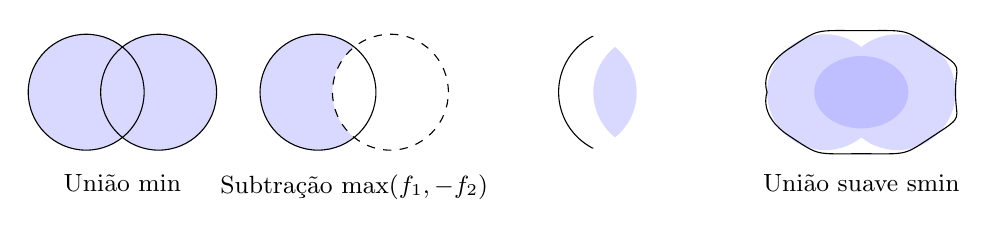
\begin{tikzpicture}[scale=0.92]
  % Union: circles A and B, filled interior
  \begin{scope}[shift={(0,0)}]
    \fill[blue!15] (0,0) circle (0.8);
    \fill[blue!15] (1.0,0) circle (0.8);
    \draw (0,0) circle (0.8);
    \draw (1.0,0) circle (0.8);
    \node[below, font=\small] at (0.5,-1.0) {União $\min$};
  \end{scope}
  % Subtraction: A minus B
  \begin{scope}[shift={(3.2,0)}]
    \fill[blue!15] (0,0) circle (0.8);
    \fill[white]   (1.0,0) circle (0.8);
    \draw (0,0) circle (0.8);
    \draw[dashed] (1.0,0) circle (0.8);
    \node[below, font=\small] at (0.5,-1.0) {Subtração $\max(f_1,-f_2)$};
  \end{scope}
  % Intersection: only overlap
  \begin{scope}[shift={(6.8,0)}]
    \clip (0,0) circle (0.8);
    \fill[blue!15] (1.0,0) circle (0.8);
    \begin{scope}[reset cm]
      \draw[shift={(6.8,0)}] (0,0) circle (0.8);
      \draw[shift={(6.8,0)}, dashed] (1.0,0) circle (0.8);
    \end{scope}
    \node[below, font=\small] at (0.5,-1.0) {Interseção $\max$};
  \end{scope}
  % Smooth union: blended boundary
  \begin{scope}[shift={(10.2,0)}]
    \fill[blue!15] (0,0) circle (0.8);
    \fill[blue!15] (1.0,0) circle (0.8);
    \fill[blue!25] (0.5,0) ellipse (0.65 and 0.5);
    \draw plot[smooth, tension=1.2] coordinates {(-0.8,0) (-0.5,-0.6) (0.5,-0.85) (1.5,-0.6) (1.8,0) (1.5,0.6) (0.5,0.85) (-0.5,0.6) (-0.8,0)};
    \node[below, font=\small] at (0.5,-1.0) {União suave $\text{smin}$};
  \end{scope}
\end{tikzpicture}
\caption{Corte transversal 2D de quatro operações CSG. A zona azul
é a região sólida $\{f<0\}$.}
\label{fig:sdf_ops}
\end{figure}

\subsection{Amostragem nos Cantos e Interpolação Trilinear}
\label{sec:sdf:corners}

A octree guarda o valor da SDF em cada um dos oito cantos de um cubo
alinhado aos eixos. Seja o cubo com canto mínimo $\mathbf{m}$
e lado de comprimento $\ell$; então o valor no canto $i$ é
\[
  d_i = f\!\left(\mathbf{m} + \ell\,\mathbf{s}_i\right),
  \qquad
  \mathbf{s}_i = \bigl(\tfrac{i_x}{1}, \tfrac{i_y}{1}, \tfrac{i_z}{1}\bigr)
    \in \{0,1\}^3,
\]
onde $(i_x, i_y, i_z)$ são os bits de $i$ (ver \S\ref{sec:octree:corners}).
A partir das oito amostras $d_0,\ldots,d_7$, podemos obter um valor
\emph{interior} usando interpolação trilinear:
\[
  f_{\text{tri}}(\mathbf{p}) =
    \sum_{k=0}^{7}
      d_k\;
      \lambda_{k_x}(t_x)\,
      \lambda_{k_y}(t_y)\,
      \lambda_{k_z}(t_z),
  \qquad
  \lambda_0(\alpha) = 1-\alpha,\quad
  \lambda_1(\alpha) = \alpha,
\]
onde $\mathbf{t} = (\mathbf{p}-\mathbf{m})/\ell\in[0,1]^3$.

\subsection{Cálculo da Normal da Superfície}
\label{sec:sdf:normal}

A normal voltada para fora em qualquer ponto $\mathbf{p}$ dentro do
cubo de um nó é calculada como o gradiente normalizado de
$f_{\text{tri}}$:
\[
  \hat{\mathbf{n}}(\mathbf{p}) =
    \frac{\nabla f_{\text{tri}}(\mathbf{p})}
         {\|\nabla f_{\text{tri}}(\mathbf{p})\|}.
\]
As componentes do gradiente são calculadas diretamente a partir da
fórmula trilinear usando a regra da cadeia, resultando numa fórmula
por eixo que soma diferenças dos valores nos cantos de faces opostas,
pesadas pelas coordenadas baricêntricas nas outras duas direções:
\begin{align*}
  \partial_x f &= \frac{1}{\ell}\Bigl[
    (1-t_y)(1-t_z)(d_4-d_0) + t_y(1-t_z)(d_6-d_2) +
    (1-t_y)t_z(d_5-d_1) + t_y t_z(d_7-d_3)
  \Bigr],
\end{align*}
com expressões análogas para $\partial_y f$ e $\partial_z f$. Esta
normal é guardada como \lstinline{Vertex::normal} e é usada tanto
para iluminação como para heurísticas de orientação baseadas na
normal da superfície.

\subsection{Posição do Vértice via QEF}
\label{sec:sdf:qef}

Dentro de cada nó de superfície, o \emph{vértice representativo} é
colocado no ponto que minimiza uma Função de Erro Quadrático (QEF),
que obriga o vértice a alinhar-se com a superfície local. Para cada
uma das 12 arestas $e$ do cubo que tenha mudança de sinal, seja
$\mathbf{p}_e$ o ponto de cruzamento da aresta (encontrado por
interpolação linear) e $\hat{\mathbf{n}}_e$ a normal interpolada
nesse ponto. O QEF minimiza
\[
  E(\mathbf{x}) = \sum_e \bigl(\hat{\mathbf{n}}_e \cdot \mathbf{x} - d_e\bigr)^2,
  \qquad d_e = \hat{\mathbf{n}}_e \cdot \mathbf{p}_e,
\]
levando ao sistema linear de mínimos quadrados
$A^\top\!A\,\mathbf{x} = A^\top b$ onde
$A^\top\!A = \sum_e \hat{\mathbf{n}}_e\hat{\mathbf{n}}_e^\top$ e
$A^\top b = \sum_e d_e\hat{\mathbf{n}}_e$. Quando a matriz tem boas
condições ($|\det(A^\top\!A)| > \epsilon$), calcula-se o minimizador
único; caso contrário, o sistema usa o centro dos pontos médios das
arestas com mudança de sinal (\lstinline{getAveragePosition}).

\subsection{Lista de Primitivas}

O motor fornece uma biblioteca de primitivas analíticas:

\begin{center}
\begin{tabular}{lll}
  \toprule
  Primitiva & Parâmetros principais & Fórmula SDF (resumo)\\
  \midrule
  Caixa (Box)        & semi-dimensões $\mathbf{b}$ & $\|\max(|\mathbf{p}|-\mathbf{b},0)\| + \min(\max(\ldots),0)$\\
  Esfera/Cápsula     & raio $r$            & $\|\mathbf{p}\| - r$, variante com segmento\\
  Cilindro           & raio $r$, altura $h$  & anel 2D + limite de altura\\
  Toro               & maior $R$, menor $r$  & $\|\,(|\mathbf{p}.xz|-R,\mathbf{p}.y)\| - r$\\
  Mapa de altitude   & raster DEM           & consulta + interpolação trilinear\\
  Ruído Perlin       & amplitude, frequência & campo de ruído stb\_perlin em camadas\\
  Voronoi 3D         & tamanho célula, semente & distância Voronoi com deformação\\
  Tira de triângulos & 4 vértices, semi-espessura & mínimo de duas SDFs de triângulo extrudido\\
  \bottomrule
\end{tabular}
\end{center}

Formas compostas são construídas juntando primitivas com um
\lstinline{WrappedSignedDistanceFunction} e combinando-as com uma
operação binária (Tabela em \S\ref{sec:sdf:ops}).

% ============================================================
\section{Octree Adaptativa — Estrutura de Dados}
\label{sec:octree}
% ============================================================

\subsection{Convenção de Indexação dos Cantos}
\label{sec:octree:corners}

Cada nó (interno ou folha) representa um cubo alinhado aos eixos.
O cubo tem oito cantos indexados de $0$ a $7$ usando três bits:
\begin{equation}
  \label{eq:corner_index}
  \text{idx}(\mathbf{p}) =
    \underbrace{[x \geq c_x]}_{\text{bit 2}} \cdot 4 \;+\;
    \underbrace{[y \geq c_y]}_{\text{bit 1}} \cdot 2 \;+\;
    \underbrace{[z \geq c_z]}_{\text{bit 0}} \cdot 1,
\end{equation}
onde $\mathbf{c} = (c_x,c_y,c_z)$ é o centro do cubo e $[\cdot]$
é o suporte de Iverson (vale 1 se a condição for verdadeira, 0 caso
contrário). As coordenadas de cada canto são:

\begin{center}
\begin{tabular}{c|c|c|c|c}
  \toprule
  Índice & $x$ & $y$ & $z$ & Bits (xyz)\\
  \midrule
  0 & min & min & min & 000 \\
  1 & min & min & max & 001 \\
  2 & min & max & min & 010 \\
  3 & min & max & max & 011 \\
  4 & max & min & min & 100 \\
  5 & max & min & max & 101 \\
  6 & max & max & min & 110 \\
  7 & max & max & max & 111 \\
  \bottomrule
\end{tabular}
\end{center}

A Figura~\ref{fig:cube_corners} mostra a disposição. Repara na
relação: inverter o bit $k$ de um índice faz a transição para o canto
vizinho ao longo do eixo $k$. Por exemplo, o canto 3 (011) e o canto
7 (111) diferem apenas no bit 2, por isso estão ligados por uma
aresta ao longo do eixo $x$.

\begin{figure}[htb]
\centering
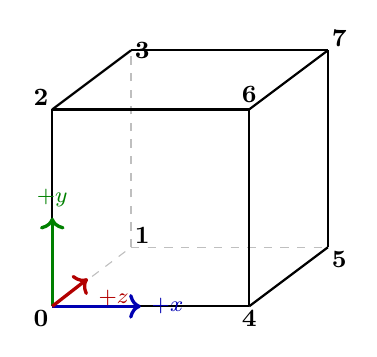
\begin{tikzpicture}[scale=2.5, thick, font=\small]
  \coordinate (C0) at (0.00, 0.00);
  \coordinate (C1) at (0.40, 0.30);
  \coordinate (C2) at (0.00, 1.00);
  \coordinate (C3) at (0.40, 1.30);
  \coordinate (C4) at (1.00, 0.00);
  \coordinate (C5) at (1.40, 0.30);
  \coordinate (C6) at (1.00, 1.00);
  \coordinate (C7) at (1.40, 1.30);

  \draw[gray!50, dashed, thin] (C0) -- (C1);
  \draw[gray!50, dashed, thin] (C1) -- (C3);
  \draw[gray!50, dashed, thin] (C1) -- (C5);

  \draw (C0) -- (C4);
  \draw (C0) -- (C2);
  \draw (C4) -- (C6);
  \draw (C2) -- (C6);
  \draw (C4) -- (C5);
  \draw (C5) -- (C7);
  \draw (C6) -- (C7);
  \draw (C2) -- (C3);
  \draw (C3) -- (C7);

  \node[below left, inner sep=1pt]  at (C0) {$\mathbf{0}$};
  \node[above right, inner sep=1pt] at (C1) {$\mathbf{1}$};
  \node[above left, inner sep=1pt]  at (C2) {$\mathbf{2}$};
  \node[right, inner sep=1pt]       at (C3) {$\mathbf{3}$};
  \node[below, inner sep=1pt]       at (C4) {$\mathbf{4}$};
  \node[below right, inner sep=1pt] at (C5) {$\mathbf{5}$};
  \node[above, inner sep=2pt]       at (C6) {$\mathbf{6}$};
  \node[above right, inner sep=1pt] at (C7) {$\mathbf{7}$};

  \draw[->, blue!70!black, very thick]
    (C0) -- ++(0.45,0) node[right, font=\footnotesize]{$+x$};
  \draw[->, green!50!black, very thick]
    (C0) -- ++(0,0.45) node[above, font=\footnotesize]{$+y$};
  \draw[->, red!70!black, very thick]
    (C0) -- ++(0.18, 0.14) node[below right, font=\footnotesize]{$+z$};
\end{tikzpicture}
\caption{Numeração dos cantos do cubo. Bits: bit~2 = $x\geq c_x$,
bit~1 = $y\geq c_y$, bit~0 = $z\geq c_z$.
As arestas a tracejado estão ocultas nesta vista.}
\label{fig:cube_corners}
\end{figure}

\subsection{As Doze Arestas do Cubo}
\label{sec:octree:edges}

As 12 arestas alinhadas aos eixos de um cubo são guardadas como pares
de índices de cantos:

\begin{center}
\small
\begin{tabular}{c|c|l}
  \toprule
  Índice da aresta & Par de cantos & Eixo e coordenadas fixas\\
  \midrule
  0  & $\{0,1\}$ & eixo $z$ em $(x_{\min}, y_{\min})$\\
  1  & $\{1,3\}$ & eixo $y$ em $(x_{\min}, z_{\max})$\\
  2  & $\{2,3\}$ & eixo $z$ em $(x_{\min}, y_{\max})$\\
  3  & $\{0,2\}$ & eixo $y$ em $(x_{\min}, z_{\min})$\\
  4  & $\{4,5\}$ & eixo $z$ em $(x_{\max}, y_{\min})$\\
  5  & $\{5,7\}$ & eixo $y$ em $(x_{\max}, z_{\max})$\\
  6  & $\{6,7\}$ & eixo $z$ em $(x_{\max}, y_{\max})$\\
  7  & $\{4,6\}$ & eixo $y$ em $(x_{\max}, z_{\min})$\\
  8  & $\{0,4\}$ & eixo $x$ em $(y_{\min}, z_{\min})$\\
  9  & $\{1,5\}$ & eixo $x$ em $(y_{\min}, z_{\max})$\\
  10 & $\{2,6\}$ & eixo $x$ em $(y_{\max}, z_{\min})$\\
  11 & $\{3,7\}$ & eixo $x$ em $(y_{\max}, z_{\max})$\\
  \bottomrule
\end{tabular}
\end{center}

\noindent
Uma mudança de sinal na aresta $e$ (ou seja, $d_{e_0} < 0 \neq
d_{e_1} < 0$ ou vice-versa) significa que a iso-superfície atravessa
essa aresta, o que desencadeia a emissão de um polígono surface-net
(\S\ref{sec:itriangles}).

\subsection{Estrutura de um Nó}

Cada nó da octree (\lstinline{OctreeNode}) guarda:
\begin{itemize}[leftmargin=2em]
  \item \lstinline{float sdf[8]} — valores SDF medidos nos oito cantos do cubo.
  \item \lstinline{Vertex vertex} — o vértice de superfície representativo
    (posição, normal, coordenada de textura, índice de pincel/material).
  \item \lstinline{uint blockId} — índice para um alocador de blocos que
    aponta para o \lstinline{ChildBlock} (8 ponteiros para filhos), ou nulo
    se for folha.
  \item \lstinline{uint8_t bits} — um campo de bits compacto com:
    \begin{itemize}
      \item \emph{SpaceType} (2 bits): \lstinline{Empty}/\lstinline{Solid}/\lstinline{Surface}
        (Vazio/Sólido/Superfície).
      \item \emph{Simplified} (1 bit): ativo quando os filhos do nó foram
        fundidos nesta representação mais grossa.
      \item \emph{Chunk} (1 bit): marca a raiz de um pedaço (chunk) de
        envio para a GPU.
      \item \emph{Leaf} (1 bit): não existem filhos.
    \end{itemize}
  \item \lstinline{uint version} — aumenta quando a geometria de um chunk
    muda; usado para invalidar caches.
\end{itemize}

\subsection{Classificação do Tipo de Espaço}
\label{sec:octree:spacetype}

Cada nó é classificado num de três tipos, examinando
$d_0,\ldots,d_7$:
\begin{align*}
  \text{Sólido}   &: \forall i,\; d_i < 0\phantom{\text{ e }\exists j} \\
  \text{Vazio}    &: \forall i,\; d_i \geq 0\\
  \text{Superfície} &: \exists\, i,j \text{ tais que } d_i < 0
    \text{ e } d_j \geq 0
\end{align*}
(considerando $\infty$ como "não tocado", excluído de ambos os testes).
Apenas os nós \lstinline{Surface} (Superfície) têm um vértice
representativo e participam na extração da malha. Os nós Sólido e
Vazio perdem os seus filhos assim que a subárvore abaixo deles está
totalmente classificada, mantendo o uso de memória proporcional à
área da superfície.

\subsection{Modelo de Memória}

Os nós são geridos através de um alocador de blocos
(\lstinline{OctreeAllocator}), que mantém duas áreas de memória:
uma para instâncias de \lstinline{OctreeNode} e outra para
\lstinline{ChildBlock}s (arrays de 8 ponteiros para filhos). O
desenho do alocador elimina a sobrecarga de memória por nó e permite
reiniciar a octree inteira em $O(1)$. A destruição segura (com
sincronização da GPU) é feita com \emph{fences} em vez de libertação
imediata.

\subsection{Hierarquia de Chunks e Threads}

A hierarquia da octree tem dois níveis especiais:
\begin{description}
  \item[Nós chunk] Nós cujo lado do cubo $\ell$ satisfaz
    $0.5\ell_{\mathrm{chunk}} < \ell \leq \ell_{\mathrm{chunk}}$.
    Não são simplificados (os seus filhos ficam expandidos), e cada
    um ativa uma função de retorno \lstinline{onNodeAdded}/
    \lstinline{onNodeDeleted} que agenda um envio de geometria para
    a GPU.
  \item[Nós thread] Nós cujo cubo é suficientemente grande
    ($\ell > \ell_{\min} \cdot 16$) lançam a avaliação da subárvore
    num conjunto de threads partilhado. Cada thread trabalha no seu
    próprio \lstinline{ThreadContext} (caches por thread para valores
    SDF e nós visitados) para evitar contenção.
\end{description}

% ============================================================
\section{Operações CSG: \texttt{apply}, \texttt{expand} e \texttt{shape}}
\label{sec:shape}
% ============================================================

O ponto de entrada para CSG é \lstinline{Octree::apply}, que agrupa
todos os passos de modificação: expansão dinâmica, descida recursiva
e agendamento de envio para a GPU. O grafo de chamadas é:

\begin{center}
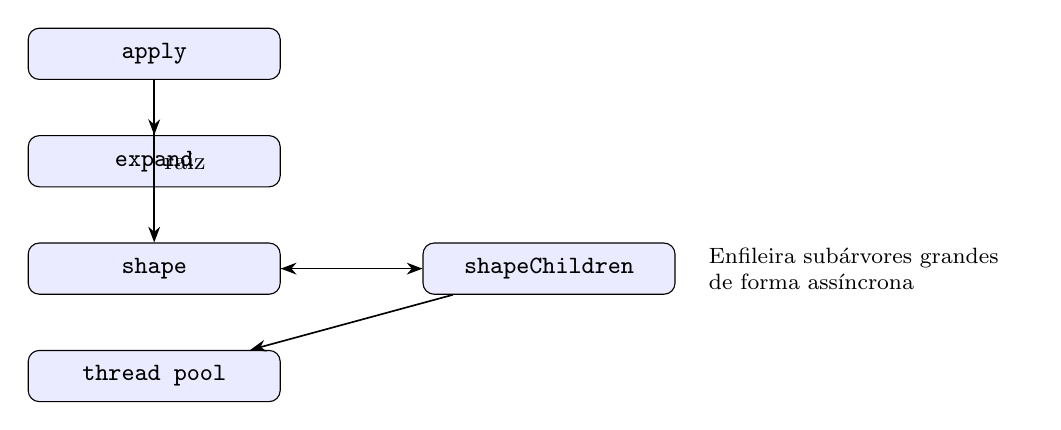
\begin{tikzpicture}[
    box/.style={draw, rounded corners, fill=blue!8,
                minimum width=3.2cm, minimum height=0.65cm,
                font=\small\ttfamily},
    arr/.style={->, >=Stealth, semithick}
  ]
  \node[box] (apply)   {\textbf{apply}};
  \node[box, below=0.7cm of apply]  (expand) {expand};
  \node[box, below=0.7cm of expand] (shape)  {shape};
  \node[box, right=1.8cm of shape]  (shapeC) {shapeChildren};
  \node[box, below=0.7cm of shape]  (thread) {thread pool};
  \draw[arr] (apply) -- (expand);
  \draw[arr] (apply) -- node[right, font=\small]{raiz} (shape);
  \draw[arr, bend right=25] (shape) -- (shapeC);
  \draw[arr, bend right=25] (shapeC) -- (shape);
  \draw[arr] (shapeC) -- (thread);
  \node[draw=none, right=0.3cm of shapeC, font=\footnotesize,
        text width=4cm, align=left]
    {Enfileira subárvores grandes\\de forma assíncrona};
\end{tikzpicture}
\end{center}

\subsection{Expansão Dinâmica (\texttt{expand})}

A raiz da octree pode não conter inicialmente todo o domínio da SDF.
\lstinline{expand} faz crescer a árvore duplicando repetidamente o
cubo do mundo até que \lstinline{function->isContained} devolva
verdadeiro. Cada duplicação:
\begin{enumerate}
  \item Calcula em que octante do novo cubo (duplicado) a raiz antiga
    se encontra (usa o centro da SDF para escolher o octante
    complementar: \lstinline{i ^ 0x7}).
  \item Aloca um novo nó raiz e um novo \lstinline{ChildBlock}, e
    coloca a raiz antiga como filho $i$.
  \item Atualiza os limites guardados (\lstinline{min},
    \lstinline{length}).
\end{enumerate}
Esta operação é idempotente (pode repetir-se sem efeitos colaterais)
e rápida: faz apenas $O(\log R)$ alocações de nós para um fator de
expansão $R$.

\subsection{Descida Recursiva (\texttt{shape})}
\label{sec:shape:shape}

\lstinline{shape} é a função recursiva principal. Dado um quadro de
nó $(\textit{node}, \textit{cube}, \textit{level}, \textit{sdf}[8],
\textit{brushIndex})$, ela:

\begin{algorithm}[H]
\caption{\lstinline{shape}(quadro, args)}
\label{alg:shape}
\begin{algorithmic}[1]
\State $\text{shapeSDF} \leftarrow \text{avaliaShapeSDF}(\text{quadro})$
\If{$\text{quadro.isLeaf}$}
  \State $\text{resultSDF} \leftarrow \text{args.operation}(\text{quadro.sdf}, \text{shapeSDF})$
  \State classifica $\text{resultType}$
\Else
  \If{$\text{args.function.check(cubo)} = \text{Disjoint}$}
    \State $\text{resultSDF} \leftarrow \text{quadro.sdf}$ \Comment{no-op, a forma não atinge este cubo}
  \Else
    \State $\text{shapeChildren}(\text{quadro})$ \Comment{desce para os 8 filhos}
    \State agrega tipos dos filhos $\to$ $\text{resultType}$
  \EndIf
\EndIf
\If{$\text{resultType} = \text{Surface}$}
  \State aloca nó se necessário
  \State $\text{node.vertex.position} \leftarrow \text{getAveragePosition}(\text{resultSDF})$
  \State $\text{node.vertex.normal} \leftarrow \nabla f(\text{position})$
  \If{$\text{isLeaf}$}
    \State $\text{brushIndex} \leftarrow \text{painter.paint}(\text{vertex})$
  \Else
    \State tenta $\text{simplificação}$ (\S\ref{sec:shape:simplify})
    \State liga filhos no \lstinline{ChildBlock} do nó
  \EndIf
\EndIf
\State escreve $\text{resultType}$, $\text{resultSDF}$, $\text{isSimplified}$, $\text{brushIndex}$ no nó
\If{$\text{isChunk}$ e $\text{resultType} = \text{Surface}$}
  \State chama \lstinline{onNodeAdded} (envio para GPU)
\EndIf
\end{algorithmic}
\end{algorithm}

\paragraph{Composição da SDF.}
Em cada nó, a SDF da forma é avaliada nos 8 cantos do cubo através
da interface \lstinline{WrappedSignedDistanceFunction::distance}
(com uma cache opcional a nível de canto). O resultado é combinado
com a SDF atual do nó usando a operação binária fornecida pelo
utilizador:
\[
  d_i^{\text{resultado}} = \text{op}(d_i^{\text{atual}},\; d_i^{\text{forma}}).
\]

\paragraph{Propagação da SDF para filhos.}
Quando um nó filho ainda não existe, os valores SDF nos seus 8 cantos
têm de ser derivados do pai. Isto é feito por
\lstinline{SDF::getChildSDF}: os oito cantos do cubo filho (que estão
dentro do cubo pai) são interpolados a partir dos valores
$d_0,\ldots,d_7$ do pai usando interpolação trilinear. Isto evita
ter que reavaliar a primitiva SDF (que pode ser cara).

\paragraph{Alocação de nós.}
Se um resultado de superfície for calculado para uma posição onde não
existe nenhum nó (por exemplo, quando uma nova pincelada cria uma
região antes vazia), um novo \lstinline{OctreeNode} é alocado da
pool, inicializado com o centro do cubo como posição temporária do
vértice, e refinado com o minimizador QEF.

\subsection{Simplificação}
\label{sec:shape:simplify}

Depois de todos os oito filhos terem sido processados, a rotina
\lstinline{Simplifier::simplify} tenta fundi-los no nó pai. O teste
tem três condições, cada uma das quais pode vetar a simplificação:

\begin{enumerate}
  \item \textbf{Uniformidade da textura.} Se a texturização estiver
    ativada, todos os filhos de superfície devem ter o mesmo índice
    de pincel. Qualquer fronteira de textura bloqueia a simplificação
    para preservar as arestas dos materiais.
  \item \textbf{Filhos todos simplificados.} Todos os filhos de
    superfície devem estar eles próprios simplificados (ou seja,
    recursivamente fundidos abaixo deles).
  \item \textbf{Erro máximo da SDF.} Para cada filho de superfície,
    a SDF do pai \emph{re-interpolada} (avaliada nos cantos do filho
    a partir dos $d_0,\ldots,d_7$ do pai) é comparada com a SDF real
    do filho. Se o erro ponto a ponto exceder $10\%$ do lado do cubo
    pai:
    \[
      |d_{\text{pai-interp}}(c_j) - d_{\text{filho}}(c_j)| >
        0.1\,\ell_{\text{pai}},
    \]
    a geometria do filho é detalhada demais para ser representada
    fielmente a uma resolução mais grossa, e a simplificação é
    rejeitada.
\end{enumerate}

\noindent
Se a simplificação for bem sucedida, o bit \emph{simplified} do nó
pai é ativado, os filhos são mantidos na árvore mas a sua geometria
é \emph{representada} pelo pai para efeitos de renderização. Os nós
de fronteira de chunk nunca são simplificados para manter uma
granularidade consistente de envio para a GPU.

\subsection{Paralelismo}

Quando \lstinline{shapeChildren} encontra um filho cujo lado do cubo
excede $16 \cdot \ell_{\min}$, a subárvore desse filho é colocada
numa fila de um \lstinline{ThreadPool} com
\lstinline{std::thread::hardware_concurrency} threads. Cada
trabalhador recebe o seu próprio \lstinline{ThreadContext} que
contém:
\begin{itemize}
  \item Uma cache \lstinline{robin_map} por subárvore para avaliações
    SDF (evita cálculos repetidos de distância dentro de uma
    subárvore).
  \item Uma cache por subárvore para consultas de
    \lstinline{getNodeAt}.
\end{itemize}
A coordenação ao nível do pai acontece via \lstinline{std::future}:
depois de lançar as oito threads potenciais, o pai espera por todos
os futuros antes de agregar os resultados dos filhos.

% ============================================================
\section{Extração da Malha Surface Nets: \texttt{iterateTriangles}}
\label{sec:itriangles}
% ============================================================

\subsection{Visão Geral e Comparação com Marching Cubes}

O \emph{Marching Cubes}~\cite{lorensen87} é um método
\emph{primal}: para cada célula que atravessa a superfície, emite
um triângulo consultando uma tabela pré-calculada com 15 casos
topológicos baseados nos sinais dos 8 cantos. Os vértices ficam nas
arestas da célula. O método é simples e robusto, mas produz malhas
blocais (degraus) e não consegue lidar naturalmente com várias
células a partilhar uma aresta em diferentes níveis de LOD.

O \emph{contorno dual}~\cite{ju02} e as \emph{surface
nets}~\cite{gibson98} são métodos \emph{duais}. Em vez de colocar
vértices nas arestas, colocam um vértice \emph{no interior} de cada
célula de superfície e ligam vértices vizinhos através de faces
partilhadas entre células. A grande vantagem é que as posições dos
vértices podem ser otimizadas (via QEF) para reproduzir arestas
vivas. A implementação aqui usa a formulação surface nets:

\begin{quote}
  \emph{Para cada aresta alinhada aos eixos que atravessa a
  superfície, emite um polígono cujos cantos são os vértices
  representativos das quatro células à volta dessa aresta.}
\end{quote}

\noindent O resultado é uma malha fechada (manifold) com orientação
correta, que se adapta naturalmente ao LOD da octree sem precisar de
preencher rachas explicitamente.

\subsection{Iteração de Arestas e Deteção de Mudança de Sinal}

\lstinline{iterateTriangles(from, fromCube, handler)} é chamada uma
vez para cada nó de superfície simplificado \lstinline{from}. Itera
sobre todas as 12 arestas de \lstinline{fromCube}. Para a aresta
$e = \{e_0, e_1\}$, uma mudança de sinal é detetada por:
\[
  \text{mudancaSinal}(e) \iff
    (d_{e_0} < 0) \neq (d_{e_1} < 0),
  \quad
  d_{e_k} = \texttt{from->sdf}[e_k].
\]
Apenas arestas com mudança de sinal são processadas; as restantes
são ignoradas.

\subsection{Segmentação de Arestas em Fronteiras de LOD}
\label{sec:itriangles:segseg}

Num grelha uniforme, cada aresta tem exatamente duas células vizinhas
por direção transversal, dando quatro células no total. Numa octree
adaptativa, as células vizinhas podem estar em diferentes níveis de
LOD: a aresta de uma célula fina pode sobrepor-se apenas parcialmente
à aresta de uma célula grossa. Cada aresta deve portanto ser dividida
em sub-segmentos, um por região contígua de cobertura uniforme de
células.

\begin{figure}[htb]
\centering
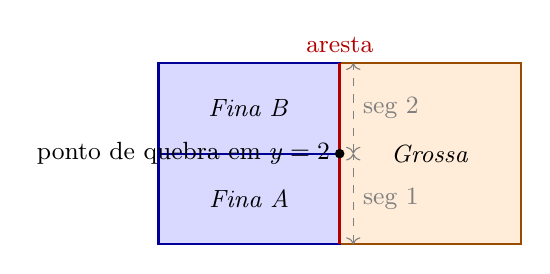
\begin{tikzpicture}[scale=1.15, font=\small]
  \fill[orange!15] (0,1) rectangle (2,3);
  \draw[orange!60!black, thick] (0,1) rectangle (2,3);
  \node at (1, 2) {\textit{Grossa}};

  \fill[blue!15] (-2,1) rectangle (0,2);
  \draw[blue!60!black, thick] (-2,1) rectangle (0,2);
  \node at (-1, 1.5) {\textit{Fina A}};

  \fill[blue!15] (-2,2) rectangle (0,3);
  \draw[blue!60!black, thick] (-2,2) rectangle (0,3);
  \node at (-1, 2.5) {\textit{Fina B}};

  \draw[very thick, red!70!black] (0,1) -- (0,3)
    node[above, red!70!black] {aresta};

  \draw[<->, dashed, black!50] (0.15,1) -- (0.15,2)
    node[midway, right] {seg 1};
  \draw[<->, dashed, black!50] (0.15,2) -- (0.15,3)
    node[midway, right] {seg 2};

  \fill[black] (0,2) circle (1.5pt) node[left]{ponto de quebra em $y=2$};
\end{tikzpicture}
\caption{Fronteira de LOD ao longo de uma aresta alinhada aos eixos.
A aresta (vermelho) é partilhada por duas células finas de um lado
e uma célula grossa do outro. O \texttt{collectBreaks} insere a
fronteira da célula em $y=2$ como ponto de quebra, dividindo a aresta
em dois sub-segmentos, cada um produzindo um polígono independente.}
\label{fig:lod_boundary}
\end{figure}

\lstinline{collectBreaks} é um procedimento recursivo que insere
pontos de quebra em todas as coordenadas de fronteira de células ao
longo da aresta (Algoritmo~\ref{alg:breaks}). Funciona amostrando
um ponto médio no intervalo atual, consultando as quatro células
à volta e extraindo os limites mínimo/máximo dos seus cubos ao longo
do eixo da aresta. Qualquer coordenada de fronteira que esteja
estritamente dentro do intervalo e ainda não esteja na lista é
adicionada. O procedimento chama-se recursivamente para cada
sub-intervalo, parando na profundidade~64 ou quando o intervalo é
menor que $2\varepsilon$.

\begin{algorithm}[H]
\caption{\lstinline{collectBreaks}(aresta, inicio, fim, quebras)}
\label{alg:breaks}
\begin{algorithmic}[1]
\If{$\text{profundidade} > 64$ \textbf{ou} $\text{fim} - \text{inicio} \leq 2\varepsilon$}
  \Return
\EndIf
\State $\text{meio} \leftarrow \tfrac{\text{inicio}+\text{fim}}{2}$
\For{$q \in \{0,1,2,3\}$}
  \State $\text{celula} \leftarrow \text{findCellAt}(\text{quadrantSample}(\text{aresta}, \text{meio}, q))$
  \State adiciona $\text{celula.cube.min}[\text{eixo}]$ e $\text{celula.cube.max}[\text{eixo}]$ a quebras
\EndFor
\For{cada sub-intervalo entre quebras adjacentes}
  \State $\text{collectBreaks}(\text{aresta, sub.inicio, sub.fim, quebras})$
\EndFor
\end{algorithmic}
\end{algorithm}

\subsection{Amostragem por Quadrantes}
\label{sec:itriangles:quadrants}

Cada sub-segmento é processado por \lstinline{emitSegment}. As quatro
células à volta do segmento são encontradas consultando a célula num
ponto de amostra que está deslocado \emph{logo para dentro} de cada
quadrante em redor do eixo da aresta.

Dado um segmento com eixo $a$ e coordenadas fixas $(u_0, v_0)$ nos
dois eixos perpendiculares, o quadrante $q$ é amostrado em:
\[
  \mathbf{p}_q = \bigl(t_{\text{meio}}, u_0 \oplus \varepsilon_u,\,
  v_0 \oplus \varepsilon_v\bigr)_a,
  \qquad (s_u, s_v) = \text{quadrantSigns}(a, q),
\]
onde $t_{\text{meio}}$ é o ponto médio do segmento ao longo do eixo
$a$, $u_0 \oplus \varepsilon_u = \texttt{nextafter}(u_0,\pm\infty)$
dependendo de $s_u$, e os sinais dos quadrantes seguem o padrão da
Tabela~\ref{tab:quad_signs}.

\begin{table}[htb]
\centering
\caption{Tabela de sinais dos quadrantes: $(s_u, s_v)$ para cada eixo
e índice de quadrante, definindo a ordem CCW (sentido anti-horário)
quando vista da direção positiva do eixo.}
\label{tab:quad_signs}
\begin{tabular}{c|cccc}
\toprule
Eixo & $q=0$ & $q=1$ & $q=2$ & $q=3$ \\
\midrule
$x$ (eixos $u{=}y,\, v{=}z$) & $(-,-)$ & $(-,+)$ & $(+,+)$ & $(+,-)$\\
$y$ (eixos $u{=}x,\, v{=}z$) & $(-,-)$ & $(+,-)$ & $(+,+)$ & $(-,+)$\\
$z$ (eixos $u{=}x,\, v{=}y$) & $(-,-)$ & $(-,+)$ & $(+,+)$ & $(+,-)$\\
\bottomrule
\end{tabular}
\end{table}

As quatro células dos quadrantes são encontradas por
\lstinline{findCellAt}, que desce na octree a partir da raiz até ao
nó de superfície simplificado mais profundo que contém o ponto de
amostra. Se alguma das quatro células não for um nó de superfície
(ou não estiver simplificada), o segmento é ignorado: não há
superfície para emitir.

\begin{figure}[htb]
\centering
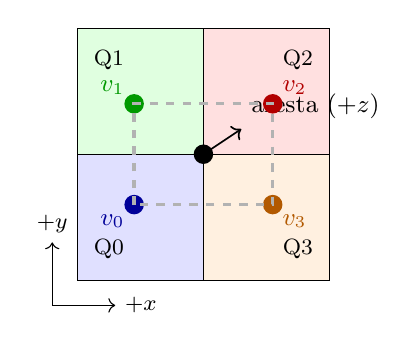
\begin{tikzpicture}[scale=1.6, font=\small]
  \fill[blue!12]  (-1,-1) rectangle (0,0);  % Q0: x-, y-
  \fill[green!12] (-1, 0) rectangle (0,1);  % Q1: x-, y+
  \fill[red!12]   (0,  0) rectangle (1,1);  % Q2: x+, y+
  \fill[orange!12](0, -1) rectangle (1,0);  % Q3: x+, y-

  \draw (-1,-1) rectangle (0,0);
  \draw (-1, 0) rectangle (0,1);
  \draw ( 0, 0) rectangle (1,1);
  \draw ( 0,-1) rectangle (1,0);

  \fill[black] (0,0) circle (2.2pt);
  \draw[->, semithick] (0,0) -- (0.3, 0.2) node[above right]{aresta ($+z$)};

  \fill[blue!60!black]  (-0.55, -0.4) circle (2.2pt) node[below left, blue!60!black]{$v_0$};
  \fill[green!60!black] (-0.55,  0.4) circle (2.2pt) node[above left, green!60!black]{$v_1$};
  \fill[red!70!black]   ( 0.55,  0.4) circle (2.2pt) node[above right, red!70!black]{$v_2$};
  \fill[orange!70!black]( 0.55, -0.4) circle (2.2pt) node[below right, orange!70!black]{$v_3$};

  \draw[very thick, dashed, gray!60]
    (-0.55,-0.4) -- (-0.55,0.4) -- (0.55,0.4) -- (0.55,-0.4) -- cycle;

  \node at (-0.75, -0.75) {\footnotesize Q0};
  \node at (-0.75,  0.75) {\footnotesize Q1};
  \node at ( 0.75,  0.75) {\footnotesize Q2};
  \node at ( 0.75, -0.75) {\footnotesize Q3};

  \draw[->] (-1.2, -1.2) -- (-0.7, -1.2) node[right]{\footnotesize $+x$};
  \draw[->] (-1.2, -1.2) -- (-1.2, -0.7) node[above]{\footnotesize $+y$};
\end{tikzpicture}
\caption{Amostragem por quadrantes para uma aresta no eixo $z$
(o ponto ao centro, a entrar na página). Quatro células à volta
(uma por quadrante) contribuem cada uma com um vértice representativo
$v_0,\ldots,v_3$. O anel poligonal resultante (tracejado) forma a
face dual.}
\label{fig:surface_nets_quad}
\end{figure}

\subsection{Regra de Propriedade}
\label{sec:itriangles:ownership}

Quando as quatro células partilham a \emph{mesma} célula ao mesmo LOD
(uma grelha uniforme), qualquer uma delas poderia ser responsável por
emitir o polígono. A regra de propriedade garante que cada polígono
é emitido exatamente uma vez, designando a célula \emph{mais fina}
(a mais pequena) como a proprietária:

\begin{quote}
  $\text{proprietário} = \argmin_{q} \ell(\text{célula}_q)$,
  onde empates são desfeitos lexicograficamente pelo canto mínimo
  do cubo, e depois pelo endereço do ponteiro.
\end{quote}

\lstinline{emitSegment} compara o proprietário encontrado com
\lstinline{from}. Se \lstinline{owner $\neq$ from}, a função retorna
sem emitir, adiando o polígono para a célula que \emph{é} a mais
fina. Isto garante que o polígono é emitido exatamente uma vez por
fronteira geométrica, independentemente de quantas vezes
\lstinline{iterateTriangles} é chamada (uma vez por nó de superfície).

\subsection{Construção do Anel Poligonal e Deduplicação}
\label{sec:itriangles:dedup}

As quatro células dos quadrantes são inseridas no array do polígono
por ordem de quadrante ($q=0,1,2,3$). Antes da inserção, são
aplicados dois passos de deduplicação:

\begin{enumerate}
  \item \textbf{Dedup de células adjacentes.} Se a célula atual é o
    mesmo nó (ou tem a mesma posição do vértice a menos de
    $\varepsilon$) que a entrada anterior, é ignorada. Isto colapsa
    células consecutivas idênticas em fronteiras de LOD degeneradas.
  \item \textbf{Dedup cabeça-cauda.} Se a primeira e a última entrada
    se referem ao mesmo nó (ou posições coincidentes), a última
    entrada é removida para evitar uma aresta de fecho degenerada.
  \item \textbf{Dedup todos-pares.} Uma verificação final $O(n^2)$
    (sobre no máximo 4 entradas) descarta o polígono inteiro se duas
    entradas não adjacentes forem idênticas, o que produziria um
    polígono auto-intersecionante ou degenerado.
\end{enumerate}

Após a deduplicação, o polígono tem 2, 3 ou 4 entradas. Tamanho~1 é
impossível após a verificação todos-pares. Tamanho~2 corresponde a
uma aresta degenerada (duas células colineares) e é ignorado.

\paragraph{Rotação para UV fiável.}
Após a deduplicação, o polígono é rodado ciclicamente para que
\lstinline{from} (o proprietário / célula mais fina) apareça no
índice~0. Isto é necessário para o mapeamento UV: o Tesselator usa
\lstinline{polygon[0].normal} para selecionar o plano de projeção
triplanar, e apenas a normal da célula mais fina (calculada a partir
da SDF de resolução total) é fiável em fronteiras de LOD curvas.

\subsection{Determinação da Orientação pelo Sinal da SDF}
\label{sec:itriangles:winding}

A orientação correta do polígono (para que a face frontal seja
visível de fora do sólido) tem de ser determinada para cada polígono.
Duas abordagens ingénuas falham:
\begin{description}
  \item[Produto externo geométrico] Calcular o produto externo de
    duas arestas do polígono e comparar com a normal estimada da
    superfície. Falha para \emph{quads não planares}: em fronteiras
    de LOD, quatro células com diferentes níveis de refinamento
    geralmente não formam um quad planar; os dois sub-triângulos do
    leque têm produtos externos em direções opostas, por isso uma
    única decisão de inversão acerta um e erra o outro.
  \item[Comparação com a normal do vértice] Comparar
    $\hat{\mathbf{n}}_0$ (a normal do vértice polígono[0]) com o
    produto externo geométrico. Falha quando polígono[0] é uma célula
    vizinha grossa cuja normal é uma média ampla sobre uma região
    grande, podendo diferir $>90^\circ$ da verdadeira direção local
    da superfície.
\end{description}

A abordagem \emph{autoritária} é derivar a orientação diretamente da
direção da mudança de sinal da SDF:

\begin{align*}
  d_0 &= f_{\text{tri}}(\mathbf{p}_{\text{início}},\;
          \text{proprietário.cubo}), \\
  d_1 &= f_{\text{tri}}(\mathbf{p}_{\text{fim}},\;
          \text{proprietário.cubo}).
\end{align*}

Os dois pontos $\mathbf{p}_{\text{início}}$ e $\mathbf{p}_{\text{fim}}$
estão na linha do eixo, no início e no fim do sub-segmento atual.
Por construção, $\text{sinal}(d_0) \neq \text{sinal}(d_1)$.

\begin{figure}[htb]
\centering
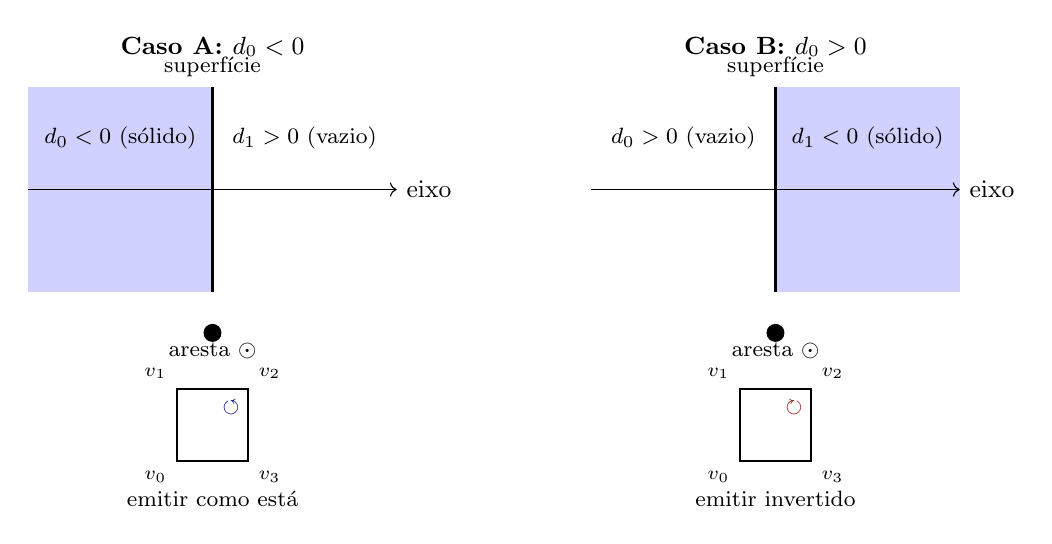
\begin{tikzpicture}[scale=1.3, font=\small]
  %--- Case 1: d0 < 0 (solid at start, surface faces +axis) ---
  \begin{scope}[shift={(0,0)}]
    \fill[blue!18] (-1.8,-1.0) rectangle (0, 1.0);
    \fill[white]   (0,-1.0)    rectangle (1.8, 1.0);
    \draw[very thick] (0,-1.0) -- (0,1.0)
      node[above, font=\footnotesize]{superfície};
    \draw[->] (-1.8,0) -- (1.8,0) node[right]{eixo};
    \node at (-0.9, 0.5) {\footnotesize $d_0 < 0$ (sólido)};
    \node at ( 0.9, 0.5) {\footnotesize $d_1 > 0$ (vazio)};
    \fill[black] (0,-1.4) circle (2.5pt);
    \node[below, font=\footnotesize] at (0,-1.4) {aresta $\odot$};
    \begin{scope}[shift={(0,-2.3)}]
      \draw[thick, ->]
        (-0.35,-0.35) node[below left, font=\scriptsize]{$v_0$} --
        (-0.35, 0.35) node[above left, font=\scriptsize]{$v_1$} --
        ( 0.35, 0.35) node[above right, font=\scriptsize]{$v_2$} --
        ( 0.35,-0.35) node[below right, font=\scriptsize]{$v_3$} --
        cycle;
      \node[below, font=\footnotesize] at (0,-0.55) {emitir como está};
      \node[above right, font=\scriptsize, color=blue!60!black] at (0,0) {$\circlearrowleft$};
    \end{scope}
    \node[above, font=\bfseries\small] at (0, 1.2) {Caso A: $d_0 < 0$};
  \end{scope}

  %--- Case 2: d0 > 0 (empty at start, surface faces -axis) ---
  \begin{scope}[shift={(5.5,0)}]
    \fill[white]   (-1.8,-1.0) rectangle (0, 1.0);
    \fill[blue!18] (0,-1.0)    rectangle (1.8, 1.0);
    \draw[very thick] (0,-1.0) -- (0,1.0)
      node[above, font=\footnotesize]{superfície};
    \draw[->] (-1.8,0) -- (1.8,0) node[right]{eixo};
    \node at (-0.9, 0.5) {\footnotesize $d_0 > 0$ (vazio)};
    \node at ( 0.9, 0.5) {\footnotesize $d_1 < 0$ (sólido)};
    \fill[black] (0,-1.4) circle (2.5pt);
    \node[below, font=\footnotesize] at (0,-1.4) {aresta $\odot$};
    \begin{scope}[shift={(0,-2.3)}]
      \draw[thick, ->]
        (-0.35,-0.35) node[below left, font=\scriptsize]{$v_0$} --
        ( 0.35,-0.35) node[below right, font=\scriptsize]{$v_3$} --
        ( 0.35, 0.35) node[above right, font=\scriptsize]{$v_2$} --
        (-0.35, 0.35) node[above left, font=\scriptsize]{$v_1$} --
        cycle;
      \node[below, font=\footnotesize] at (0,-0.55) {emitir invertido};
      \node[above right, font=\scriptsize, color=red!60!black] at (0,0) {$\circlearrowright$};
    \end{scope}
    \node[above, font=\bfseries\small] at (0, 1.2) {Caso B: $d_0 > 0$};
  \end{scope}
\end{tikzpicture}
\caption{Determinação da orientação pelo sinal da SDF. Preenchimento
azul = sólido ($f<0$); branco = vazio ($f>0$). O anel poligonal
(mostrado como quadrado para uma configuração de 4 células) é emitido
como está quando o sólido está no extremo inferior do eixo (Caso A),
ou invertido quando o sólido está no extremo superior (Caso B).
A inversão mantém $v_0$ (a célula proprietária) como o pivô do leque.}
\label{fig:winding}
\end{figure}

A lógica de emissão para um leque de triângulos a partir de
polígono[0]:
\[
  \text{solidoNoInicio} = (d_0 < 0).
\]
\begin{center}
\begin{tabular}{ll}
  \toprule
  \multicolumn{1}{c}{solidoNoInicio = verdadeiro} &
  \multicolumn{1}{c}{solidoNoInicio = falso}\\
  \midrule
  $(v_0, v_1, v_2)$ & $(v_0, v_2, v_1)$ \\
  $(v_0, v_2, v_3)$ & $(v_0, v_3, v_2)$ \\
  \bottomrule
\end{tabular}
\end{center}
Ambos os sub-triângulos do leque recebem a mesma inversão
autoritária, que é independente das normais dos vértices e permanece
correta mesmo quando as quatro células formam um quad não planar.

A orientação segue a convenção \texttt{VK\_FRONT\_FACE\_CLOCKWISE}
do Vulkan: quando $d_0 < 0$ (sólido no extremo inferior do eixo), a
superfície está virada para a direção positiva do eixo, e a ordem
dos quadrantes $Q_0\!\to\!Q_1\!\to\!Q_2\!\to\!Q_3$ produz um polígono
que parece estar no sentido horário quando visto de fora do sólido
(do lado positivo do eixo).

\subsection{Emissão do Leque de Triângulos}

Os triângulos são emitidos através de uma função que verifica
degenerescência:
\[
  \text{emitirTriangulo}(a, b, c) \;\text{ sse }\;
    \|a-b\| > \varepsilon, \quad \|b-c\| > \varepsilon, \quad \|c-a\| > \varepsilon.
\]
Triângulos degenerados aparecem quando várias células partilham a
mesma posição do vértice (por exemplo, dentro de uma região
perfeitamente plana), e descartá-los evita polígonos de área zero no
buffer da GPU.

Os triângulos finais são enviados para um
\lstinline{OctreeNodeTriangleHandler}, que na pipeline padrão é uma
instância de \lstinline{Tesselator}.

% ============================================================
\section{Tesselação e Mapeamento UV}
\label{sec:tesselator}
% ============================================================

A função de retorno \lstinline{Tesselator::handle(v0, v1, v2)}
recebe um triângulo e executa duas tarefas antes de o adicionar ao
buffer de geometria:

\paragraph{Filtro de pincel.}
Os três vértices devem ter um índice de pincel válido
($> \texttt{DISCARD\_BRUSH\_INDEX}$) para serem incluídos. Vértices
com $\texttt{brushIndex} = -1$ não foram pintados e são ignorados,
evitando artefactos de nós não inicializados.

\paragraph{Mapeamento UV triplanar.}
As coordenadas UV são atribuídas projetando cada posição do vértice
no plano do eixo dominante, selecionado a partir de
$v_0.\texttt{normal}$:

\[
  \text{plano}(\hat{\mathbf{n}}) =
  \begin{cases}
    0 & |n_x| > |n_y| \text{ e } |n_x| > |n_z|, \; n_x > 0\\
    1 & |n_x| > |n_y| \text{ e } |n_x| > |n_z|, \; n_x \leq 0\\
    2 & |n_y| > |n_x| \text{ e } |n_y| > |n_z|, \; n_y > 0\\
    3 & \text{(} y \text{ negativo)}\\
    4 & |n_z|\text{ dominante}, \; n_z > 0\\
    5 & \text{(} z \text{ negativo)}\\
  \end{cases}
\]

As coordenadas UV para cada plano são:
\begin{center}
\begin{tabular}{c|c}
  \toprule
  Plano & $(u, v)$ \\
  \midrule
  0 ($+x$) & $(-p_z,\; -p_y)$ \\
  1 ($-x$) & $(\phantom{-}p_z,\; -p_y)$ \\
  2 ($+y$) & $(\phantom{-}p_x,\; \phantom{-}p_z)$ \\
  3 ($-y$) & $(\phantom{-}p_x,\; -p_z)$ \\
  4 ($+z$) & $(\phantom{-}p_x,\; -p_y)$ \\
  5 ($-z$) & $(-p_x,\; -p_y)$ \\
  \bottomrule
\end{tabular}
\end{center}
Os três vértices usam o mesmo plano (determinado por $v_0$),
garantindo que não há quebras dentro de um único triângulo. A UV é
depois escalada por \lstinline{triplanarScale = 0.1f} para controlar
a densidade da repetição da textura.

\paragraph{Passagem da orientação.}
O Tesselator já não reordena vértices: a orientação correta foi
pré-determinada por \lstinline{emitSegment}
(\S\ref{sec:itriangles:winding}), por isso
\lstinline{geometry.addTriangle(v0, v1, v2)} é chamado diretamente.

% ============================================================
\section{Discussão}
\label{sec:discussion}
% ============================================================

\subsection{Malha sem Rachas nos LODs}

Uma propriedade crítica da abordagem surface nets é que não é
necessário preencher rachas explicitamente. Quando uma célula fina
e uma célula grossa partilham uma aresta, o mecanismo
\lstinline{collectBreaks} divide a aresta na fronteira da célula fina,
e a regra de propriedade atribui o polígono à célula mais fina. A
célula grossa é incluída como uma das quatro células do quadrante,
contribuindo com o seu vértice (possivelmente mais grosseiro) para
o polígono. A malha resultante é topologicamente correta e estanque
nas costuras de LOD, ao custo de quads ligeiramente não planares
perto das transições — precisamente a situação que a correção de
orientação pelo sinal da SDF resolve.

\subsection{Qualidade dos Vértices nas Transições de LOD}

Numa fronteira de LOD, as quatro células do quadrante podem ter
tamanhos de cubo muito diferentes. Os vértices representativos das
células mais grossas são posicionados com QEF sobre uma região maior,
introduzindo mais erro posicional. A qualidade da malha depende do
limiar de simplificação; limites mais apertados (distância e ângulo
menores no \lstinline{Simplifier}) produzem melhor posicionamento dos
vértices mas contagens de polígonos maiores.

\subsection{Fronteiras de Pincel / Material}

As fronteiras de material são tratadas de forma conservadora: o
simplificador rejeita a fusão quando dois filhos têm índices de
pincel diferentes. Isto garante que as transições de material são
representadas com resolução total, ao custo de uma malha mais fina
nessas regiões. Uma otimização futura poderia permitir simplificação
através de fronteiras de material quando a geometria é plana,
guardando ambos os índices de material no pai e interpolando.

\subsection{Granularidade do Paralelismo}

O esquema de threading atual lança um futuro por subárvore filha que
excede o limiar de nó thread. Isto pode criar até 8 tarefas por nó
interno, levando a uma fila grande para árvores profundas. Uma
abordagem mais controlada seria limitar a profundidade do envio
assíncrono e usar uma fila de roubo de trabalho.

\subsection{Limitações}

\begin{itemize}
  \item \textbf{Arestas vivas.} O minimizador QEF pode teoricamente
    reconstruir arestas e cantos vivos colocando o vértice na
    interseção de múltiplos planos da superfície. No entanto, o
    recurso a \lstinline{getAveragePosition} (usado quando a matriz
    QEF tem más condições) perde informação de arestas vivas.
  \item \textbf{Mudanças de topologia.} Modificações que alteram o
    género da superfície (por exemplo, perfurar um túnel) podem
    deixar estado de simplificação desatualizado em nós pai
    inalterados. É necessário um novo percurso completo das
    subárvores afetadas.
  \item \textbf{Polígonos surface-net de tamanho 2.} Polígonos
    degenerados com dois vértices são descartados silenciosamente, o
    que pode deixar pequenos buracos na malha em níveis de LOD muito
    grossos ou em características mais finas que uma célula.
\end{itemize}

% ============================================================
\section{Conclusão}
\label{sec:conclusion}
% ============================================================

Descrevemos um sistema completo de octree adaptativa para terreno SDF
com CSG em tempo real. O sistema integra quatro subsistemas
interligados: (1) uma octree alocada por blocos que guarda amostras
SDF nos cantos e um vértice de superfície de qualidade em cada nó;
(2) um percurso CSG recursivo que atualiza a octree incrementalmente
com avaliação opcional de subárvores em multi-threading e
simplificação de LOD baseada em distância e ângulo; (3) um extrator
de malha surface nets que lida com LOD não uniforme, resolve a
propriedade dos polígonos sem ambiguidade e deriva a orientação dos
triângulos apenas do sinal da SDF; e (4) um mapeador UV triplanar
que seleciona o eixo de projeção a partir do gradiente autoritário
da SDF.

A principal ideia de desenho é que o sinal da SDF nos extremos de
uma aresta é um oráculo suficiente e fiável para a orientação do
polígono — é independente das normais dos vértices (que se degradam
em níveis de LOD grossos e em quads não planares), tornando a
determinação da orientação robusta em todas as configurações de
superfície.

% ============================================================
\begin{thebibliography}{9}

\bibitem{lorensen87}
W.~E. Lorensen and H.~E. Cline.
\newblock Marching cubes: A high resolution 3d surface construction algorithm.
\newblock In \emph{ACM SIGGRAPH Computer Graphics}, volume~21(4), pages~163--169,
  1987.

\bibitem{ju02}
T.~Ju, F.~Losasso, S.~Schaefer, and J.~Warren.
\newblock Dual contouring of hermite data.
\newblock In \emph{ACM Transactions on Graphics (SIGGRAPH)}, volume~21(3),
  pages~339--346, 2002.

\bibitem{gibson98}
S.~F. F. Gibson.
\newblock Constrained elastic surface nets: generating smooth surfaces from
  binary segmented data.
\newblock In \emph{Proc. MICCAI}, pages~888--898, 1998.

\bibitem{hart96}
J.~C. Hart.
\newblock Sphere tracing: A geometric method for the antialiased ray tracing of
  implicit surfaces.
\newblock \emph{The Visual Computer}, 12(10):527--545, 1996.

\bibitem{quilez}
I.~Quilez.
\newblock Smooth minimum.
\newblock \url{https://iquilezles.org/articles/smin/}, 2013.

\end{thebibliography}

\end{document}
